\section{Multivariable Differential Calculus}

Here are examples related to differential calculus in more than one variable.

\subsection{Envelopes}

In the simplist cases, the \textbf{envelope} of a family \(\mathfrak F\) of curves is a curve \(\gamma\) that is in some sense extremal to the entire family of curves. 
What is often the case, is that every point of the curve \(\gamma\) touches exaclty one curve from the the family \(\mathfrak F\), and furthermore this touching is only tangential (i.e. they cross at an angle of zero). 
This is best illustrated with examples. 

\subsubsection{The Hyperbola as an Envelope}

\subsubsection*{The Set Up}

Consider the family \(\mathfrak F\) of straight lines in \(\mathbb R^2\), where each line crosses the x-axis and y-axis at pairs of points of the form \((s,0)\) and \((0, 1/s)\) for some \(s > 0\). 
So we see that each line is of the form \(\frac{1}{s} x + s y = 1\) for some \(s > 0\).
Some of the lines from the family are pictured in the following figure.

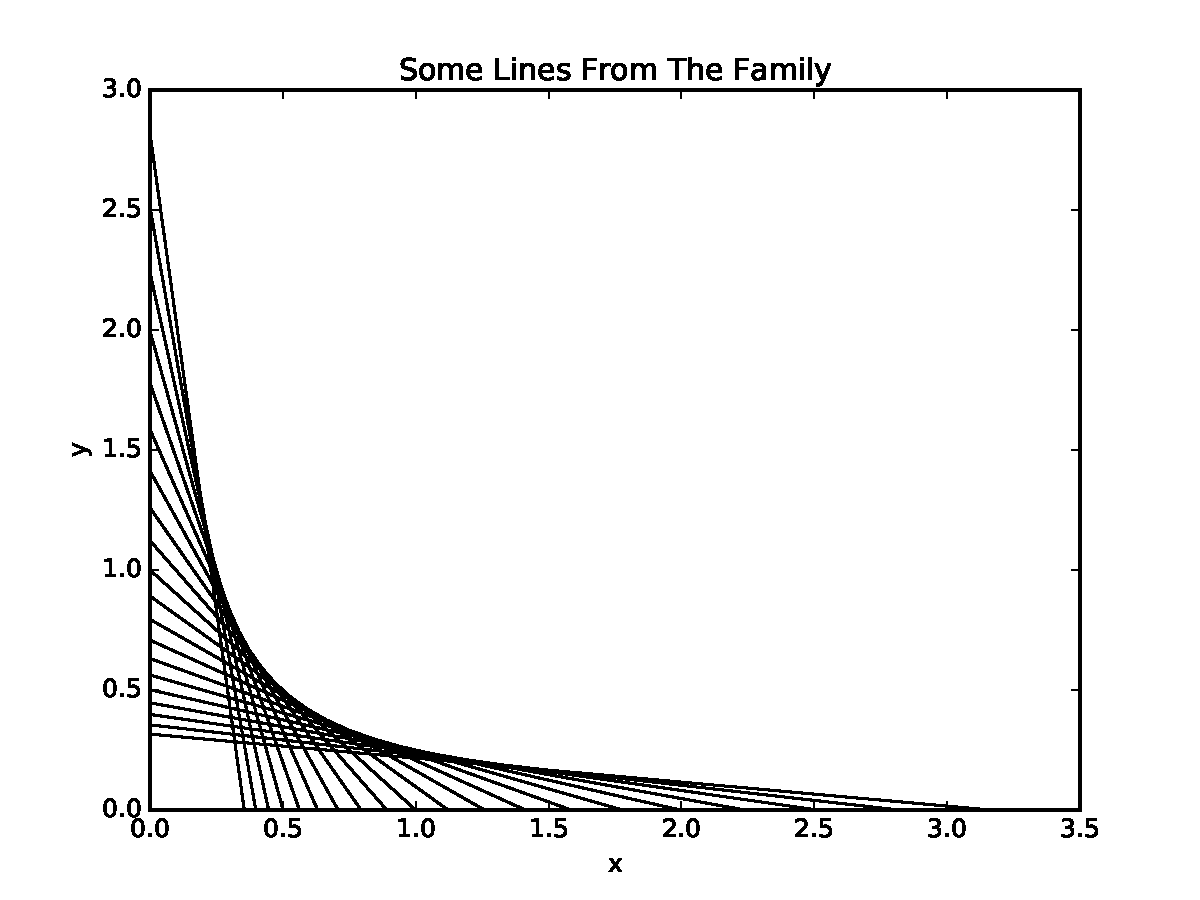
\includegraphics[width = 4.0in]{multiVarDiffCalc/hyperbolaFamily.pdf}

We can see that extemal to the family of lines is a curve concave up in the first quadrant \(\{x, y > 0\}\). In the following figure, you can see the curve superimposed with some of the lines from the family.

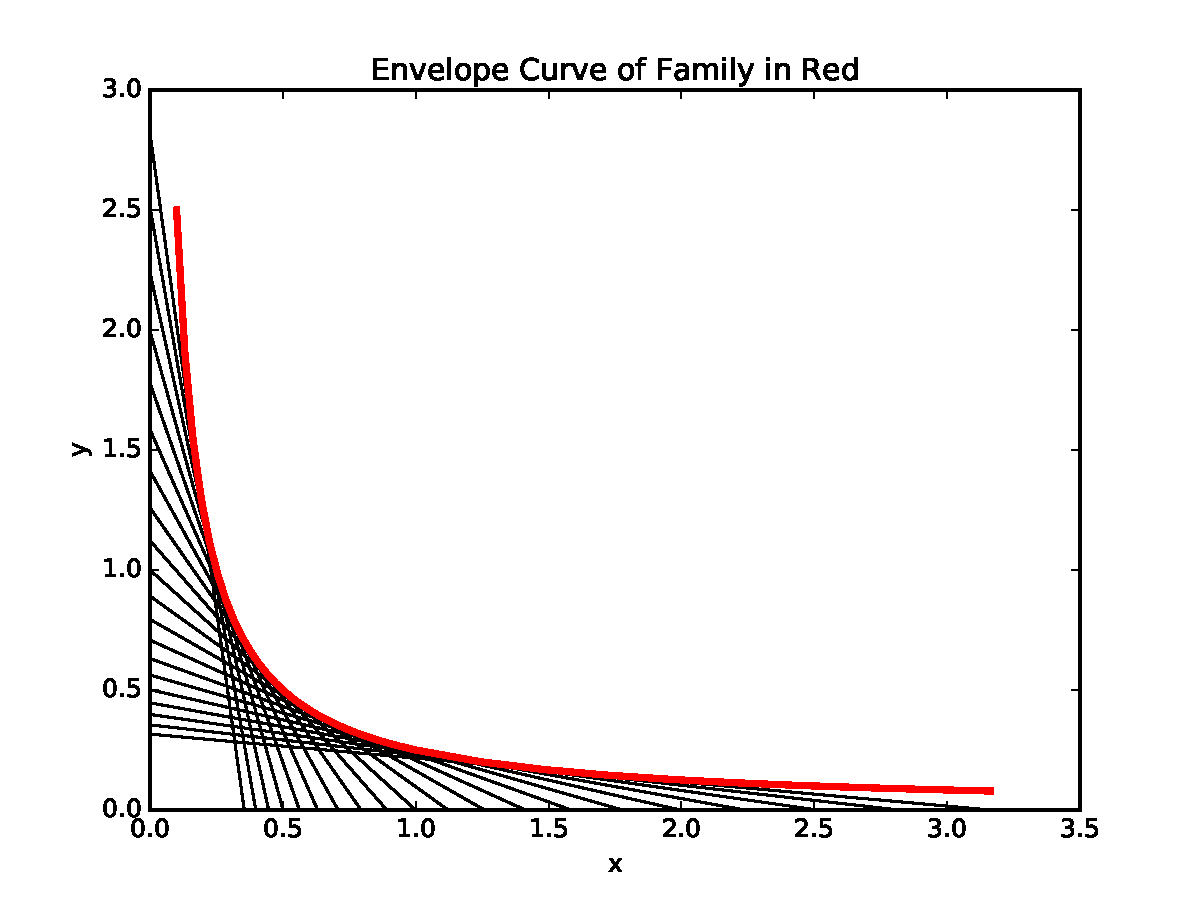
\includegraphics[width = 4.0in]{multiVarDiffCalc/hyperbolaEnvelope.pdf}

\subsubsection*{The Problem}
Let us consider computing the envelope curve \(\gamma(x)\) of the family \(\mathfrak F\). 

\subsubsection*{The Solution}

To compute the envelope curve \(\gamma(x)\), let us consider the auxilliary function
\(g(x,y,s) = \frac{1}{s} x + s y - 1\). Let us see how the Implicit Function Theorem of vector calculus let's us
use \(g(x,y, s)\) to find the exremal envelope curve \(\gamma(x)\). As we discuss this, please consider the similarities to the ordinary first derivative test.

First, consider any point \((x_0, y_0)\) NOT on the extremal envelope curve \(\gamma(x)\), but is touched by some line in \(\mathfrak F\). 
So there is some \(s_0 > 0\) such that \(\frac{1}{s_0} x_0 + s_0 y_0 = 1\); note that this is equivalent to \(g(x_0, y_0, s_0) = 0\). 
Since \((x_0, y_0)\) isn't on the boundary of the region of points touched by lines in \(\mathfrak F\), we know that for any other points \((x_1, y_1)\) close to \((x_0, y_0)\) we may find another line in \(\mathfrak F\) touching \((x_1, y_1)\). 
That is, for every \((x_1, y_1)\) close to \((x_0, y_0)\), we may find \(s_1 > 0\) such that \(g(x_1, y_1, s_1) = 0\).  

This can be summarized as saying that for all points \((x_0, y_0)\) that are touched by a line in \(\mathfrak F\) and also isn't on the envelope \(\gamma\), we can locally solve \(s = S(x,y)\) such that \(g(x, y, S(x, y)) = 0\). Now, you may begin to see the connection to the Implicit Function Theorem.

Recall that the Implicit Function Theorem can only confirm that we CAN locally solve \(s = S(x,y)\) such that \(g(x, y, S(x, y)) = 0\). However, we seek for the extremal points where we CAN'T locally solve. This is similar to the first derivative test of ordinary calculus. Technically, the first derivate test only says when a point is NOT an extemum of a function; then the candidate points for extrema are reduced to some finite list by solving for the vanishing of the derivative.

Here, we are in a similar situation. We solve for a set of candidate points that must contain our extremal curve \(\gamma\). 
It will happen to be the case that our candidate set will allow only one curve and so this must be the envelope.
However, we are being a little reckless here as we haven't proven the curve must exist; we will consider the picture to be very convincing and ignore this technical detail. 

So we seek for when we can't locally solve \(s = S(x,y)\) such that \(g(x, y, S(x, y)) = 0\). The Implicit Function Theorem tells us this will only be possible for those \((x,y,s)\) with \(g(x,y,s) = 0\) and \(\frac{\partial g}{\partial s} (x, y, s) = 0\).

So we look for
\begin{align}
0 & = \frac{\partial g}{\partial s}, \\
&  = -\frac{x}{s^2} + y
\end{align}

We wish to find an equation restricting \(x\) and \(y\); so it is most efficient to solve the above for \(s\). 
Also, from the picture it is clear that we should restrict to \(x, y > 0\). 
Therefore, for \(x, y > 0\), we have \(s = \sqrt{\frac{x}{y}}\). Plugging this into the equation for \(g(x, y, s) = 0\), we get 
\begin{equation}
\sqrt{xy} + \sqrt{xy} - 1 = 0.
\end{equation} 

Therefore, we find that the envelope curve must lie inside the set \(S = \{xy = \frac{1}{4}\}\). However, one will recognize that for each point \(x > 0\), there is only one \(y\) such that \(y \in S\). Therefore, the envelope must be this curve.

So the envelope \(\gamma(x)\) is the curve \(y = \frac{1}{4x}\) for \(x > 0\).  

\subsubsection*{Final Remark}

Note that the set \(S\) is actually a hyperbola. Therefore, the hyperbola can be realized as the envelope of a simple family of straight lines. For this reason, hyperbolas are (approximately) reproducible in "string art": art formed from
straight line segments where each segment is made by tightened string.
